\documentclass[11pt]{article}
\usepackage[margin=1in]{geometry}
\usepackage{graphicx}
\usepackage{booktabs}
\usepackage{amsmath,amssymb}
\usepackage{microtype}
\usepackage{hyperref}
\usepackage{caption}
\usepackage{longtable}
\usepackage{float}
\usepackage{textcomp}
\usepackage{tikz}
\usepackage[T1]{fontenc}
\usepackage[utf8]{inputenc}
\usepackage[numbers,sort&compress]{natbib}
\usepackage{setspace}
\onehalfspacing

\graphicspath{{../results/figures/}}

\title{Dispersion, not displacement:\\loss of alveolar epithelial state coherence in lethal COVID-19}
\author{[Author names and affiliations to be added]}
\date{\today}

\begin{document}
\maketitle

% ============================================================================
% ABSTRACT
% ============================================================================
\begin{abstract}
\noindent
The alveolar epithelium repairs itself through AT2-to-AT1 differentiation, but this process is overwhelmed in lethal COVID-19. Two geometric models could describe the resulting injury: coherent displacement of cells toward a single damaged state, or heterogeneous dispersion across multiple injury states. We tested these models using 22{,}128 alveolar epithelial cells from the Columbia/NYP COVID-19 Lung Atlas (SCP1219; 7 healthy donors, 20 COVID-19 donors), scoring eight gene programs along diffusion pseudotime and evaluating robustness through ten pre-specified ablation analyses, Harmony batch correction, an orthogonal trajectory algorithm (Palantir), and independent replication on 89{,}736 cells from 618 donors across 35 datasets.

Coherent centroid displacement was not supported (one-sided Mann--Whitney $p = 1.0$; rank-biserial $r = 0.14$ opposite to the hypothesized direction). Within-group dispersion was strongly supported (variance ratio 2.3; Levene $p < 10^{-30}$) and replicated decisively cross-cohort (variance ratio 1.65; $p \approx 10^{-137}$). COVID-19 cells were enriched at higher pseudotime (permutation $p = 0.001$; median difference $+0.048$ on a $[0,1]$ axis), a signal preserved in 27/27 leave-one-donor-out iterations, amplified 2.6-fold under Harmony batch correction, confirmed at reduced magnitude by Palantir ($+0.028$), and replicated at the donor-pseudobulk level in the independent cohort ($p = 0.002$). A KRT8\textsuperscript{+}/CLDN4\textsuperscript{+} transitional population was enriched 3.1-fold in the primary atlas but did not transfer cross-cohort under marker-threshold definitions. The fine-grained ordering of injury programs along pseudotime was sensitive to gene-list composition and is treated as hypothesis-generating.

These results support a model in which lethal COVID-19 produces dispersion-dominated loss of alveolar epithelial state coherence rather than a coherent directional shift. Within-group dispersion and donor-level trajectory direction are the most portable findings across cohorts and methods; annotation-dependent and threshold-based measures are atlas-specific.
\end{abstract}

% ============================================================================
% INTRODUCTION
% ============================================================================
\section{Introduction}

The alveolar epithelium is the functional unit of gas exchange in the lung. Two cell types sustain this function: AT1 cells, which form the thin gas-exchange barrier across approximately 95\% of the alveolar surface, and AT2 cells, which secrete pulmonary surfactant and serve as the resident stem cells of the alveolar compartment. When AT1 cells are lost to injury, AT2 cells proliferate and differentiate through a KRT8\textsuperscript{+}/CLDN4\textsuperscript{+}/SFN\textsuperscript{+} transitional state to regenerate the gas-exchange surface \citep{Barkauskas2013, Kobayashi2020, Strunz2020}. This AT2-to-AT1 differentiation axis is the primary mechanism of alveolar self-repair.

In lethal COVID-19, this regenerative system is overwhelmed. SARS-CoV-2 enters AT2 cells via ACE2, directly compromising both the surfactant system and the regenerative progenitor pool \citep{Ziegler2020, Hou2020}. A dysregulated inflammatory response inflicts further collateral damage. Autopsy studies describe diffuse alveolar damage, loss of normal architecture, and accumulation of transitional epithelial cells that are neither fully AT2 nor fully AT1 \citep{Borczuk2020, Melms2021}. Single-cell atlases of these tissues have revealed cell-type compositional changes and differentially expressed genes \citep{Melms2021, Delorey2021}, but the cluster-based approach they employ forces continuous biology into discrete bins.

A trajectory-based approach offers a more informative alternative. By treating each cell's expression profile as a position on a continuous transcriptomic manifold and ordering cells along pseudotime \citep{Haghverdi2016, Setty2019}, one can ask whether the molecular evidence is consistent with staged failure and characterize the geometry of the injury pattern. However, this approach raises a question that is rarely addressed explicitly: what is the expected \emph{shape} of epithelial injury in transcriptomic space?

Two competing geometric models make distinct predictions (Figure~\ref{fig:fig1}). Under a \textbf{coherent displacement model}, injury shifts the entire cell population away from the healthy centroid toward a single new location in gene-expression space, implying a uniform damaged state. Under a \textbf{dispersion model}, injury fans cells outward from the healthy region into a heterogeneous cloud of partially overlapping injury states, increasing within-group variance without necessarily moving the centroid. These models make opposite predictions for two standard metrics: a centroid-displacement test (significant under displacement, null under dispersion) and a variance test (null under displacement, significant under dispersion). Both models predict enrichment at higher pseudotime values under a root-in-healthy-cells design.

Here, we test these models using alveolar epithelial cells from the Columbia/NYP COVID-19 Lung Atlas \citep{Melms2021}. We pre-specified three statistical criteria --- centroid displacement, within-group dispersion, and pseudotime enrichment --- and evaluated robustness through ten ablation analyses, Harmony batch correction, an orthogonal trajectory algorithm (Palantir), and independent cross-cohort replication on 89{,}736 alveolar cells from 618 donors across 35 datasets. The result is an explicit accounting of which conclusions are robust across methodological choices, which are portable across cohorts, and which are atlas-specific.

% ============================================================================
% FIGURES - Main
% ============================================================================

\begin{figure}[htbp]
\centering
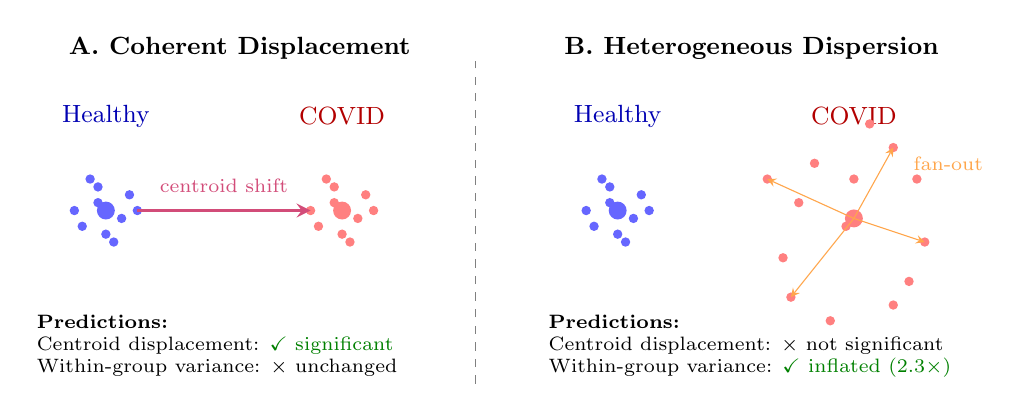
\begin{tikzpicture}[
  cell/.style={circle, inner sep=1.2pt, fill},
  healthy/.style={cell, fill=blue!60},
  covid/.style={cell, fill=red!50},
  centroid/.style={circle, draw, thick, inner sep=2pt, fill=white},
  arr/.style={->, thick, >=stealth},
  label/.style={font=\small\bfseries},
]

% --- Panel A: Coherent Displacement ---
\node[label, anchor=south] at (2.5,4.2) {A. Coherent Displacement};

% Healthy cluster (left)
\node[label, font=\small, blue!70!black] at (0.8,3.6) {Healthy};
\foreach \x/\y in {0.5/2.2, 0.7/2.5, 0.9/2.0, 1.1/2.6, 0.6/2.8, 1.0/2.3, 0.8/2.1, 1.2/2.4, 0.4/2.4, 0.7/2.7}
  \node[healthy] at (\x,\y) {};
\node[centroid, blue!60] at (0.8,2.4) {};

% COVID cluster (shifted right)
\node[label, font=\small, red!70!black] at (3.8,3.6) {COVID};
\foreach \x/\y in {3.5/2.2, 3.7/2.5, 3.9/2.0, 4.1/2.6, 3.6/2.8, 4.0/2.3, 3.8/2.1, 4.2/2.4, 3.4/2.4, 3.7/2.7}
  \node[covid] at (\x,\y) {};
\node[centroid, red!50] at (3.8,2.4) {};

% Displacement arrow
\draw[arr, purple!70, very thick] (1.2,2.4) -- (3.4,2.4);
\node[font=\scriptsize, purple!70, above] at (2.3,2.5) {centroid shift};

% Predictions
\node[font=\scriptsize, align=left, anchor=north west] at (-0.2,1.2) {
  \textbf{Predictions:}\\
  Centroid displacement: \textcolor{green!50!black}{\checkmark{} significant}\\
  Within-group variance: $\times$ unchanged
};

% --- Panel B: Heterogeneous Dispersion ---
\node[label, anchor=south] at (9,4.2) {B. Heterogeneous Dispersion};

% Healthy cluster (left)
\node[label, font=\small, blue!70!black] at (7.3,3.6) {Healthy};
\foreach \x/\y in {7.0/2.2, 7.2/2.5, 7.4/2.0, 7.6/2.6, 7.1/2.8, 7.5/2.3, 7.3/2.1, 7.7/2.4, 6.9/2.4, 7.2/2.7}
  \node[healthy] at (\x,\y) {};
\node[centroid, blue!60] at (7.3,2.4) {};

% COVID cloud (dispersed, centroid stays similar)
\node[label, font=\small, red!70!black] at (10.3,3.6) {COVID};
\foreach \x/\y in {9.5/1.3, 10.8/3.2, 9.2/2.8, 11.2/2.0, 10.0/1.0, 10.5/3.5, 9.8/3.0, 11.0/1.5, 10.2/2.2, 9.6/2.5, 10.8/1.2, 10.3/2.8, 9.4/1.8, 11.1/2.8}
  \node[covid] at (\x,\y) {};
\node[centroid, red!50] at (10.3,2.3) {};

% Fan-out arrows
\draw[arr, orange!70, thin] (10.3,2.3) -- (9.5,1.3);
\draw[arr, orange!70, thin] (10.3,2.3) -- (10.8,3.2);
\draw[arr, orange!70, thin] (10.3,2.3) -- (11.2,2.0);
\draw[arr, orange!70, thin] (10.3,2.3) -- (9.2,2.8);
\node[font=\scriptsize, orange!70] at (11.5,3.0) {fan-out};

% Predictions
\node[font=\scriptsize, align=left, anchor=north west] at (6.3,1.2) {
  \textbf{Predictions:}\\
  Centroid displacement: $\times$ not significant\\
  Within-group variance: \textcolor{green!50!black}{\checkmark{} inflated (2.3$\times$)}
};

% Divider
\draw[gray, dashed] (5.5,0.2) -- (5.5,4.3);

\end{tikzpicture}
\caption{\textbf{Competing geometric models of epithelial injury.} \textbf{(A)} Under coherent displacement, injury shifts the entire cell population toward a single new location, predicting significant centroid displacement but unchanged within-group variance. \textbf{(B)} Under heterogeneous dispersion, injury fans cells outward into a cloud of partially overlapping states, predicting increased within-group variance without net centroid displacement. Our data support model B: dispersion-dominated loss of state coherence.}
\label{fig:fig1}
\end{figure}

% ============================================================================
% RESULTS
% ============================================================================
\section{Results}

% --- 1. Cohort ---
\subsection{Cohort composition and alveolar subset validation}

We extracted 22{,}128 alveolar epithelial cells from SCP1219 by retaining cells annotated as AT1, AT2, or ECM-high epithelial in the original atlas \citep{Melms2021}: 9{,}608 AT1 cells, 11{,}341 AT2 cells, and 1{,}179 ECM-high transitional cells from 27 donors (12{,}181 cells from 7 healthy controls; 9{,}947 from 20 COVID-19 cases). Per-donor alveolar cell counts ranged from 62 to 2{,}850, and 10 of 27 donors contributed fewer than 300 cells (Supplementary Table~S5). The true inferential sample size is therefore 27 donors (7 versus 20), and we rely on donor-level analyses and leave-one-donor-out ablation throughout to ensure that no single donor drives any primary finding.

Marker-gene expression confirmed annotation quality: AT2 cells expressed \textit{SFTPC} and \textit{SFTPA1}; AT1 cells expressed \textit{AGER} and \textit{HOPX}; ECM-high transitional cells expressed \textit{KRT8} and \textit{CLDN4} at elevated levels relative to both AT1 and AT2 populations (Supplementary Table~S3). The marker profile of the ECM-high compartment is consistent with the KRT8\textsuperscript{+}/CLDN4\textsuperscript{+} damage-associated transient progenitor (DATP) population described in mouse bleomycin injury and human idiopathic pulmonary fibrosis \citep{Kobayashi2020, Strunz2020, Adams2020, Habermann2020}.

\begin{figure}[htbp]
\centering
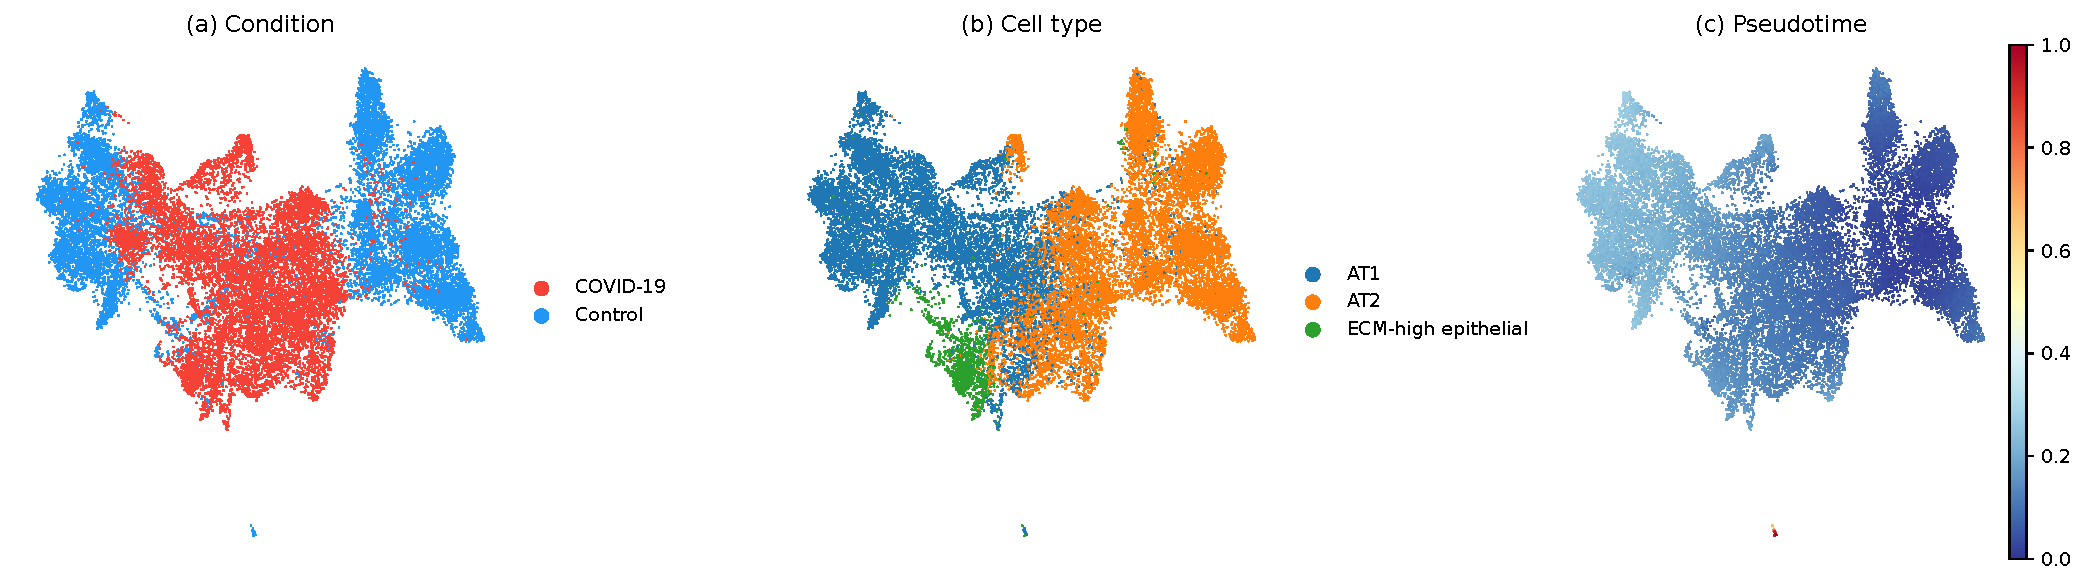
\includegraphics[width=\textwidth]{fig2_manifold.pdf}
\caption{\textbf{Alveolar epithelial manifold.} UMAP of 22,128 alveolar epithelial cells colored by condition (left), cell type annotation (center), and diffusion pseudotime (right). Pseudotime is rooted at the healthy AT2 centroid and normalized to $[0, 1]$.}
\label{fig:fig2}
\end{figure}

% --- 2. Competing models ---
\subsection{Two competing models of epithelial injury: centroid displacement fails, dispersion succeeds}\label{sec:competing}

The central question of this study is whether alveolar epithelial injury in lethal COVID-19 takes the form of coherent displacement or heterogeneous dispersion. We tested both using the same cells in the same 50-dimensional PCA space.

\paragraph{Centroid displacement was not supported.} We computed the Euclidean distance from each cell to the centroid of healthy cells in PCA space and tested whether COVID-19 cells were farther from this centroid than healthy cells (one-sided Mann--Whitney $U$, alternative COVID $>$ Healthy). The test was not significant ($U = 5.206 \times 10^7$, $p = 1.0$; rank-biserial $r = 0.14$ pointing opposite to the alternative). The median distance was 10.68 for COVID-19 cells and 11.56 for healthy cells --- COVID-19 cells were, if anything, \emph{closer} to the healthy centroid than healthy cells were to their own centroid. This result was pre-specified as one of three core criteria and the data do not support it.

\paragraph{Within-group dispersion was strongly supported.} For each condition we computed each cell's Euclidean distance to that condition's own centroid in PCA space. The variance of these distances was 33.28 in COVID-19 and 14.58 in controls (ratio 2.3). Levene's test yielded a statistic of 276.5 with $p < 10^{-30}$ (Table~\ref{tab:tab2}). COVID-19 alveolar cells occupy a markedly broader region of transcriptomic space than healthy cells, consistent with fragmentation into heterogeneous injury states rather than coherent movement to a single new state.

\paragraph{Interpretation: dispersion, not displacement.} These two results together discriminate between the competing models of Figure~\ref{fig:fig1}. The absence of centroid displacement rules out the simpler model in which all COVID-19 cells shift coherently toward one damaged phenotype. The strong dispersion signal supports the alternative model in which injury fans cells outward across multiple partially overlapping states while some cells remain near homeostatic identity. A test that measures mean displacement averages over the near-healthy and the distant subpopulations and detects neither. A test that measures within-group variance captures exactly this structure. We propose that future studies of epithelial state loss should adopt dispersion-based or trajectory-based metrics in preference to centroid-displacement tests, which implicitly assume a unimodal shift that injury biology does not produce.

% --- 3. Dispersion centerpiece ---
\subsection{Dispersion-dominated loss of state coherence is the most portable finding}\label{sec:dispersion}

The dispersion result is the strongest and most portable finding in this study. In the primary atlas, the 2.3-fold variance ratio between COVID-19 and healthy cells is the largest effect size among all tested metrics.

To evaluate cross-cohort portability, we constructed an independent replication cohort of 89{,}736 alveolar AT1/AT2 nuclei from the cellxgene census (35 datasets, 618 donors; the Melms/SCP1219 dataset was excluded by its identifier). We scored the same eight gene programs and defined an injury composite as the mean of the six non-homeostatic program scores. Levene's test on the injury composite yielded a statistic of 626.2 with $p \approx 10^{-137}$ and a variance ratio of 1.65 (COVID variance 0.0505; normal variance 0.0306). The direction and qualitative magnitude of the primary-cohort dispersion finding replicate decisively.

\paragraph{Donor-level dispersion.} At the donor level, the pattern is more nuanced. Per-donor within-donor median distance to own centroid was 7.77 for COVID-19 donors and 10.58 for healthy donors (Mann--Whitney $p = 0.999$; Levene $p = 0.071$). Individual COVID-19 donors are not more internally dispersed than individual healthy donors; rather, the cell-level dispersion signal arises from the diversity of states \emph{across} COVID-19 donors. This is consistent with a model in which each donor's cells occupy a different region of injury space, collectively producing the fan-out visible at the cell level. The within-donor dispersion bootstrap 95\% CI for the difference in medians was $[-30.7, 16.5]$, confirming that the cell-level Levene's test captures between-donor heterogeneity rather than within-donor inflation (Figure~\ref{fig:fig3}c).

\begin{figure}[htbp]
\centering
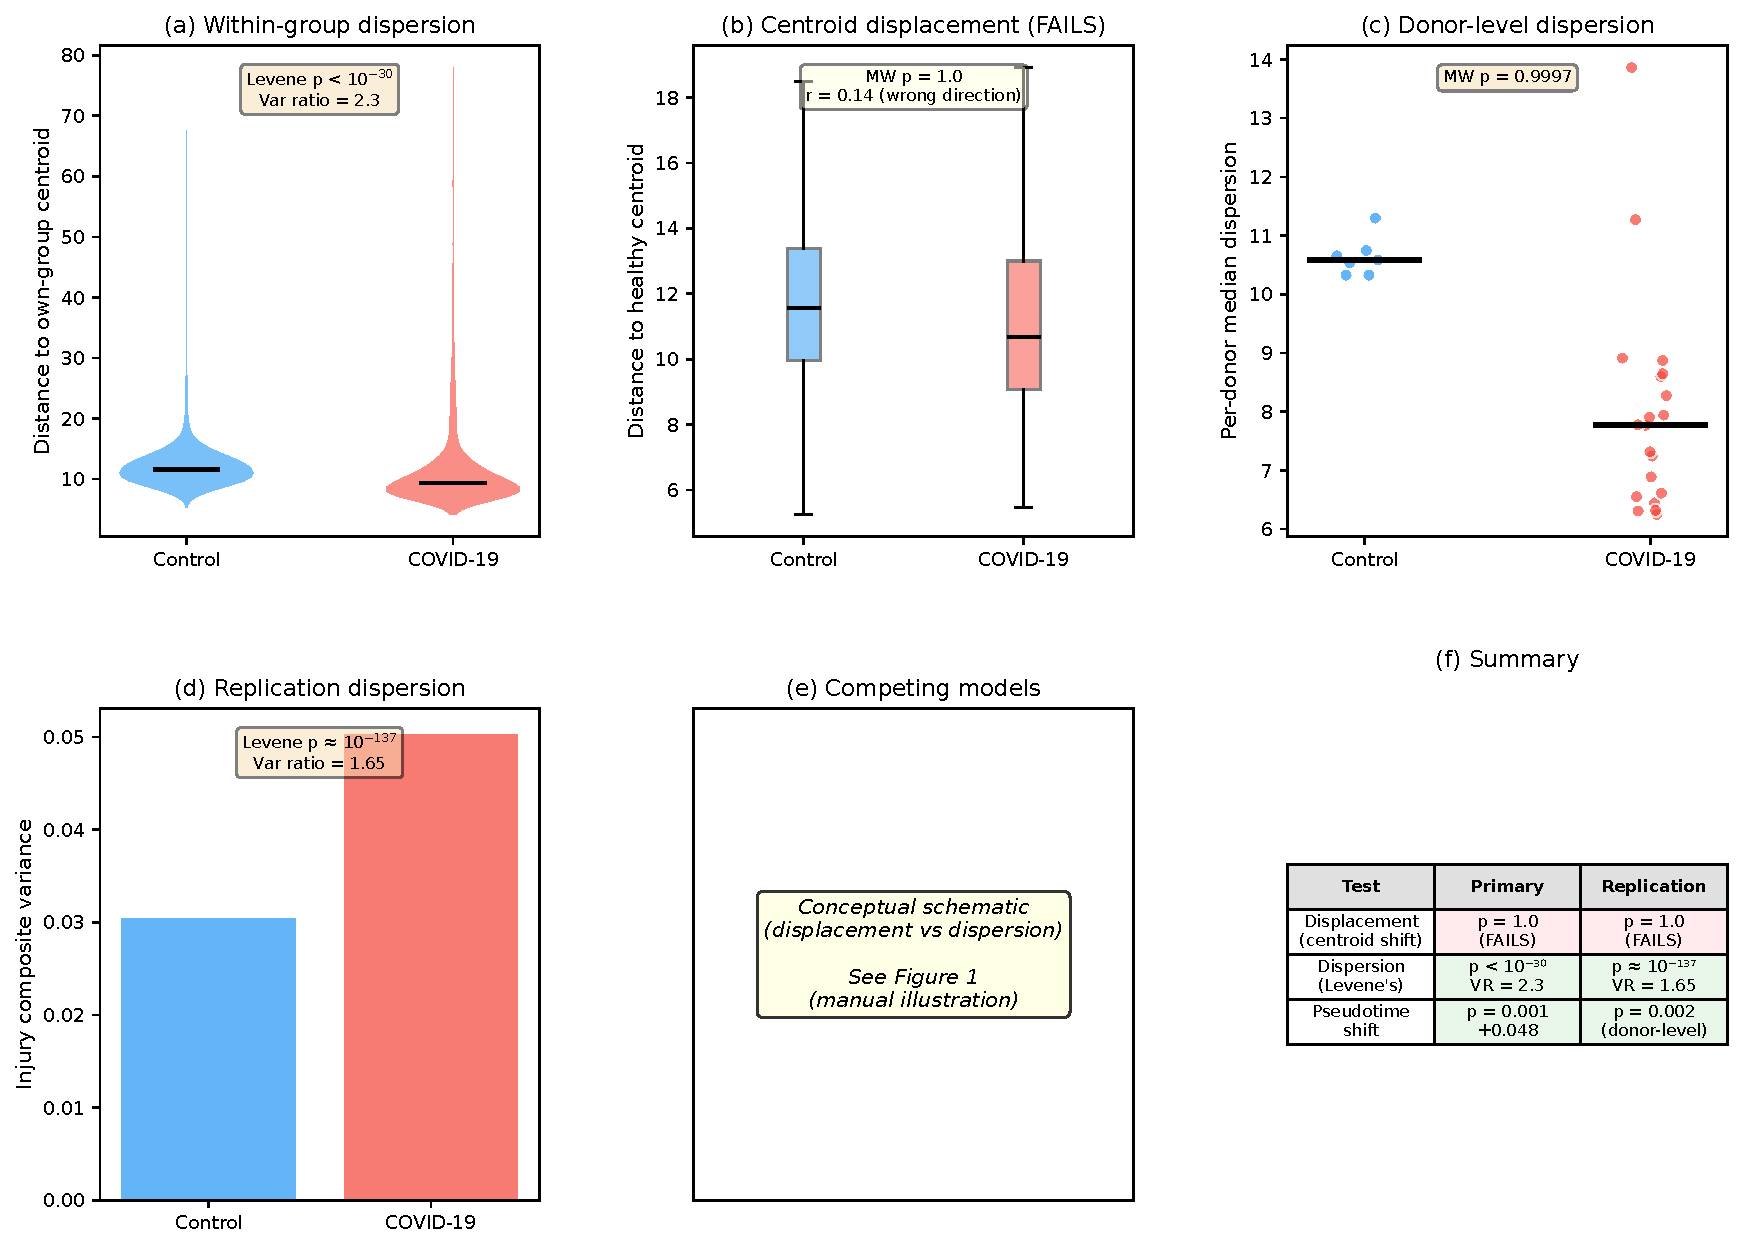
\includegraphics[width=\textwidth]{fig3_dispersion_centerpiece.pdf}
\caption{\textbf{Dispersion-dominated loss of state coherence.} \textbf{(a)} Within-group distance-to-centroid distributions for COVID-19 and healthy cells (Levene $p < 10^{-30}$; variance ratio 2.3). \textbf{(b)} Distance-to-healthy-centroid distributions (displacement test; Mann--Whitney $p = 1.0$). \textbf{(c)} Donor-level within-donor dispersion: COVID-19 donors are not individually more dispersed; the cell-level signal arises from between-donor heterogeneity. \textbf{(d)} Replication cohort dispersion (Levene $p \approx 10^{-137}$; variance ratio 1.65). \textbf{(e)} Summary statistics table.}
\label{fig:fig3}
\end{figure}

% --- 4. Pseudotime shift ---
\subsection{COVID-19 cells are enriched at higher pseudotime along a donor-robust injury axis}

We constructed a transcriptomic manifold (3{,}000 HVGs, 50-component PCA, $k$-nearest-neighbor graph with $k = 15$, 15-component diffusion map) and computed diffusion pseudotime rooted at the cell nearest the healthy AT2 centroid in diffusion-component space, min-max normalized to $[0, 1]$.

\paragraph{Pseudotime shift.} COVID-19 cells were shifted toward higher pseudotime (median 0.111 versus 0.063; observed difference $+0.048$). A 1{,}000-iteration permutation test (condition labels shuffled, median difference recomputed) placed the null distribution tightly at zero (mean $6.0 \times 10^{-5}$, std $1.24 \times 10^{-3}$); the observed value exceeded all permutations ($p = 0.000999$). The shift is modest in absolute magnitude (approximately 5\% of the normalized range) but statistically robust.

\paragraph{Donor-level robustness.} Leave-one-donor-out analysis (27 iterations) preserved the direction of the shift in every iteration, with magnitude ranging from 0.028 to 0.202 and the bulk of iterations clustering between 0.047 and 0.086. No single donor was necessary for the pseudotime shift to remain positive.

All 20 COVID-19 donors had median pseudotime $\geq 0.087$, while 5 of 7 control donors had median pseudotime $< 0.090$. No COVID-19 donor had a median pseudotime below the lowest healthy-donor median.

\paragraph{Harmony batch correction amplifies the shift.} Harmony \citep{Korsunsky2019} with \texttt{donor\_id} as batch key converged in three iterations and yielded a pseudotime shift of $+0.125$, approximately 2.6-fold larger than the uncorrected value. This amplification is biologically interpretable: donor-level batch effects, confounded with condition in this autopsy-versus-organ-donor cohort, act as within-donor clustering forces in PCA space. Removing that within-donor clustering while preserving between-condition structure unmasks a larger condition-associated shift. The fact that batch correction \emph{strengthens} rather than weakens the signal is strong evidence that the pseudotime shift is not a donor-effect artifact.

\paragraph{Palantir cross-validation.} Palantir \citep{Setty2019} on the same manifold and root cell returned a median pseudotime shift of $+0.028$ between conditions, of the same sign as diffusion pseudotime and comparable in magnitude. The program-ordering correlation with the primary analysis was $\rho = 0.48$. This cross-algorithm agreement on the direction and approximate magnitude of the shift indicates that the signal is a property of the underlying manifold rather than an artifact of one algorithm.

\paragraph{Donor-level replication.} In the independent replication cohort, the cell-level one-sided Mann--Whitney test on the injury composite returned $p = 1.0$ (consistent with the cell-level centroid-displacement failure in the primary cohort). However, pseudobulking to donor-level medians and testing 43 COVID donors versus 575 control donors yielded $p = 0.002$ in the expected direction. This pattern --- cell-level unimodal-shift tests fail, donor-level aggregated tests succeed --- mirrors the primary cohort and reinforces the view that cell-level displacement tests are not the appropriate instrument for this class of biology.

\begin{figure}[htbp]
\centering
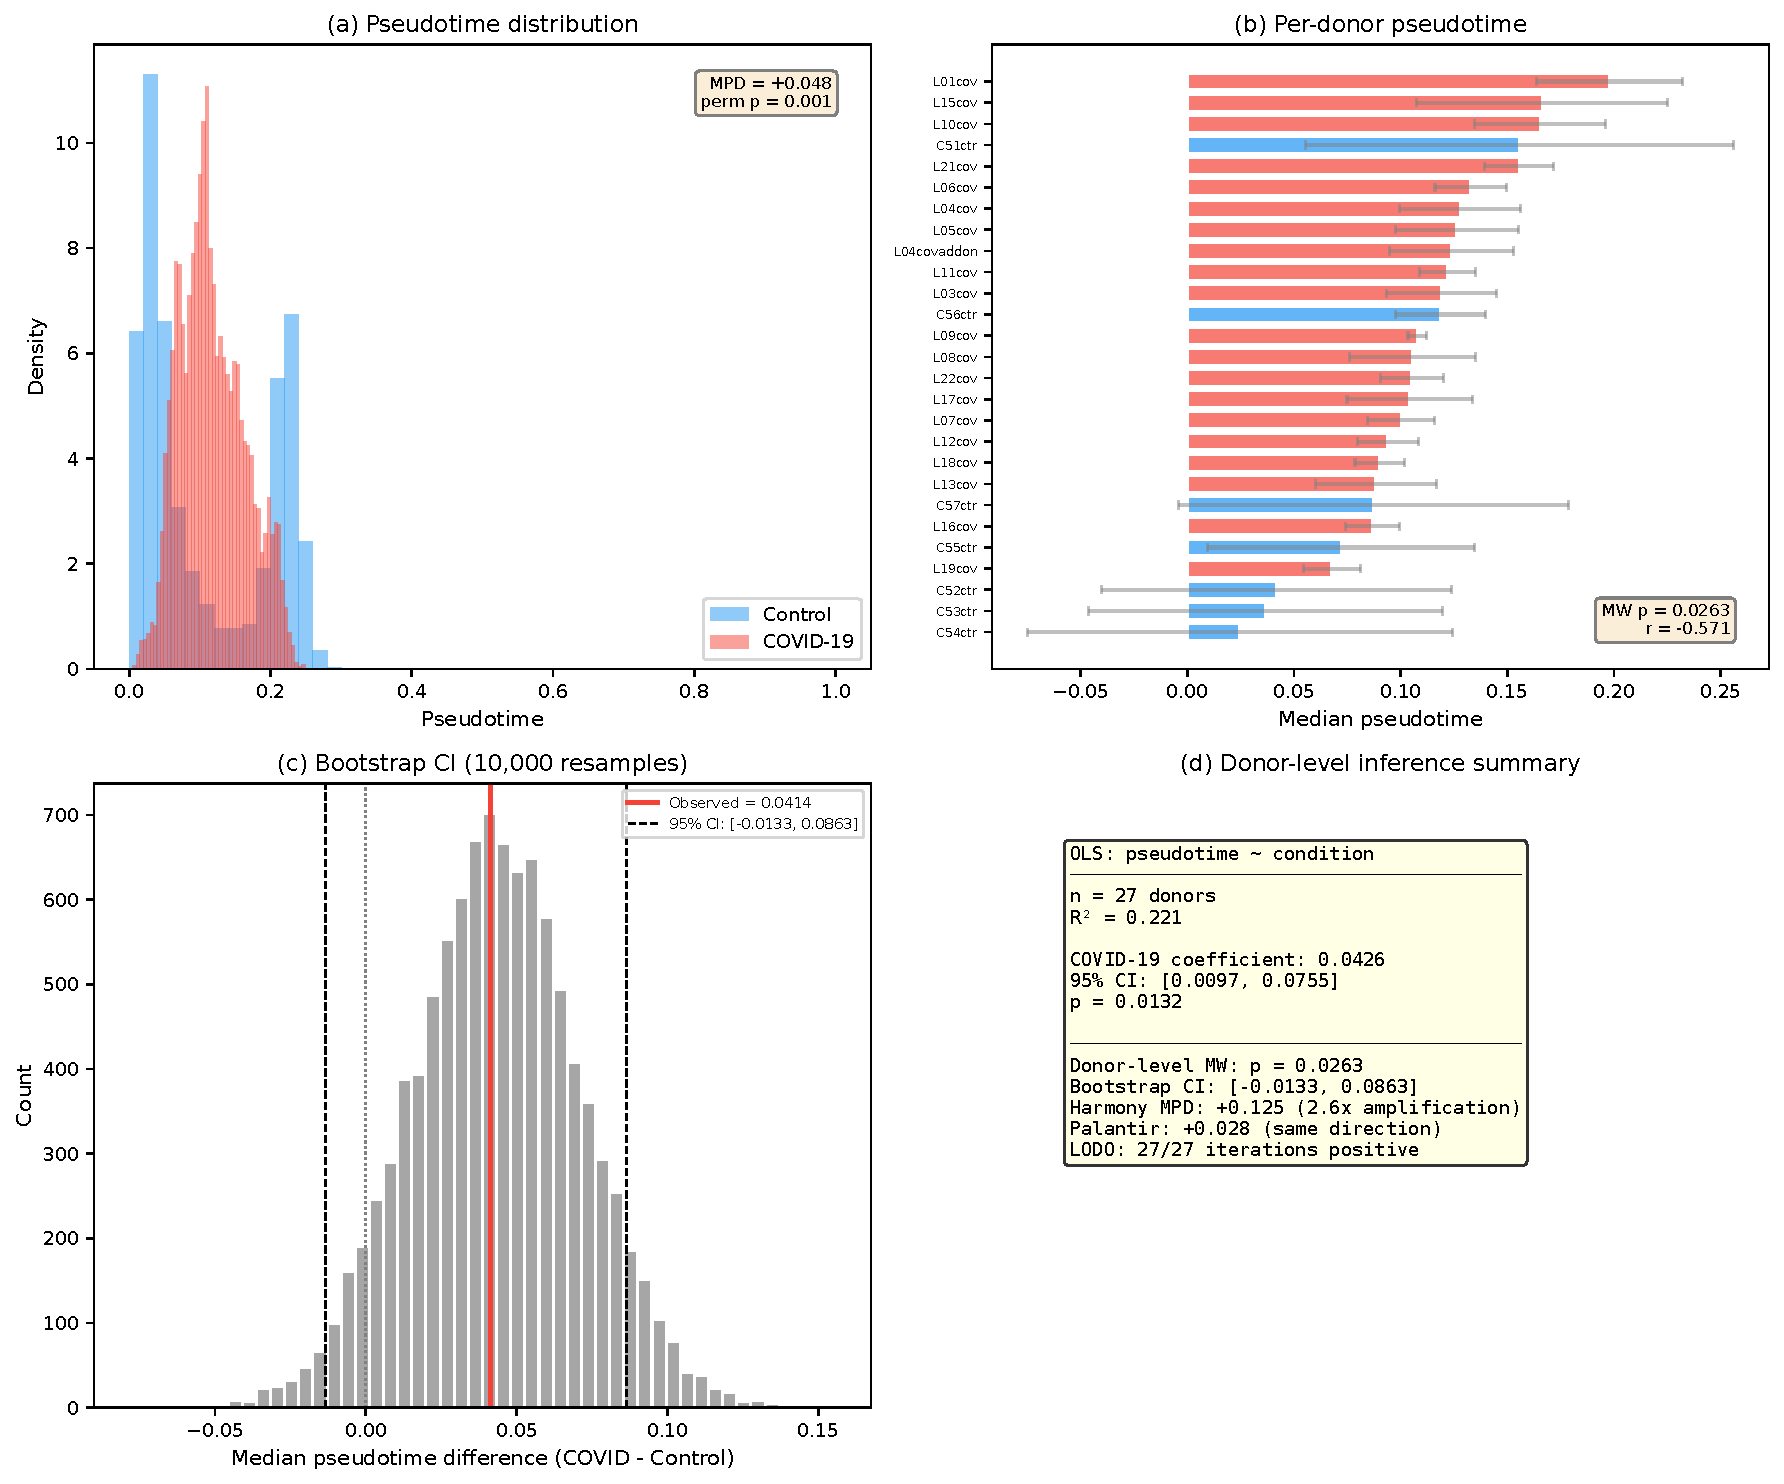
\includegraphics[width=\textwidth]{fig4_donor_pseudotime.pdf}
\caption{\textbf{Donor-level pseudotime analysis.} \textbf{(a)} Pseudotime density distributions by condition. \textbf{(b)} Per-donor median pseudotime (bars), sorted by value. \textbf{(c)} Bootstrap distribution (10,000 replicates) for the difference in donor-level median pseudotime between conditions; 95\% CI $[-0.013, 0.086]$. \textbf{(d)} OLS model summary: coefficient $+0.043$ ($p = 0.013$; $R^2 = 0.22$).}
\label{fig:fig4}
\end{figure}

% --- 5. Transitional compartment ---
\subsection{A KRT8\textsuperscript{+}/CLDN4\textsuperscript{+} transitional compartment is enriched in the primary atlas but is not a portable cross-cohort signature}

The ECM-high transitional population was enriched 3.1-fold in COVID-19 relative to controls (848/9{,}947 COVID cells [8.5\%] versus 331/12{,}181 control cells [2.7\%]; $\chi^2$ $p < 10^{-30}$). These cells occupied intermediate pseudotime positions (mean $\approx 0.3$--$0.5$), expressed \textit{KRT8}, \textit{CLDN4}, and partial AT1 markers (Supplementary Table~S3), and are consistent with damage-associated transient progenitors described in mouse lung injury \citep{Kobayashi2020, Strunz2020} and aberrant basaloid cells described in human IPF \citep{Adams2020, Habermann2020}. Their enrichment in COVID-19 and their intermediate pseudotime position are together consistent with accumulation of cells that initiated AT2-to-AT1 repair but did not complete it. This interpretation is correlational; we have a cross-sectional snapshot, not a lineage trace.

\paragraph{Cross-cohort portability of marker-threshold DATP calling fails.} In the independent replication cohort, we defined DATP-positive cells as those with simultaneously positive expression of KRT8 and CLDN4 (log-normalized count $> 0$ for both). The fraction was 22.9\% in COVID-19 versus 47.6\% in controls (fold enrichment $0.48\times$; $\chi^2$ $p \approx 10^{-228}$), the opposite direction from the primary atlas. This failure reflects cross-cohort non-equivalence of simple marker-threshold calls: study-specific normalization, capture efficiency, and ontology labeling all affect how many cells cross a fixed expression threshold. We therefore report DATP enrichment as a primary-atlas observation, not a cross-cohort-validated finding. A full-transcriptome classifier trained on the Melms transitional-cell signature would be the appropriate portable alternative; the 84-gene replication panel is too narrow for such a classifier.

\begin{figure}[htbp]
\centering
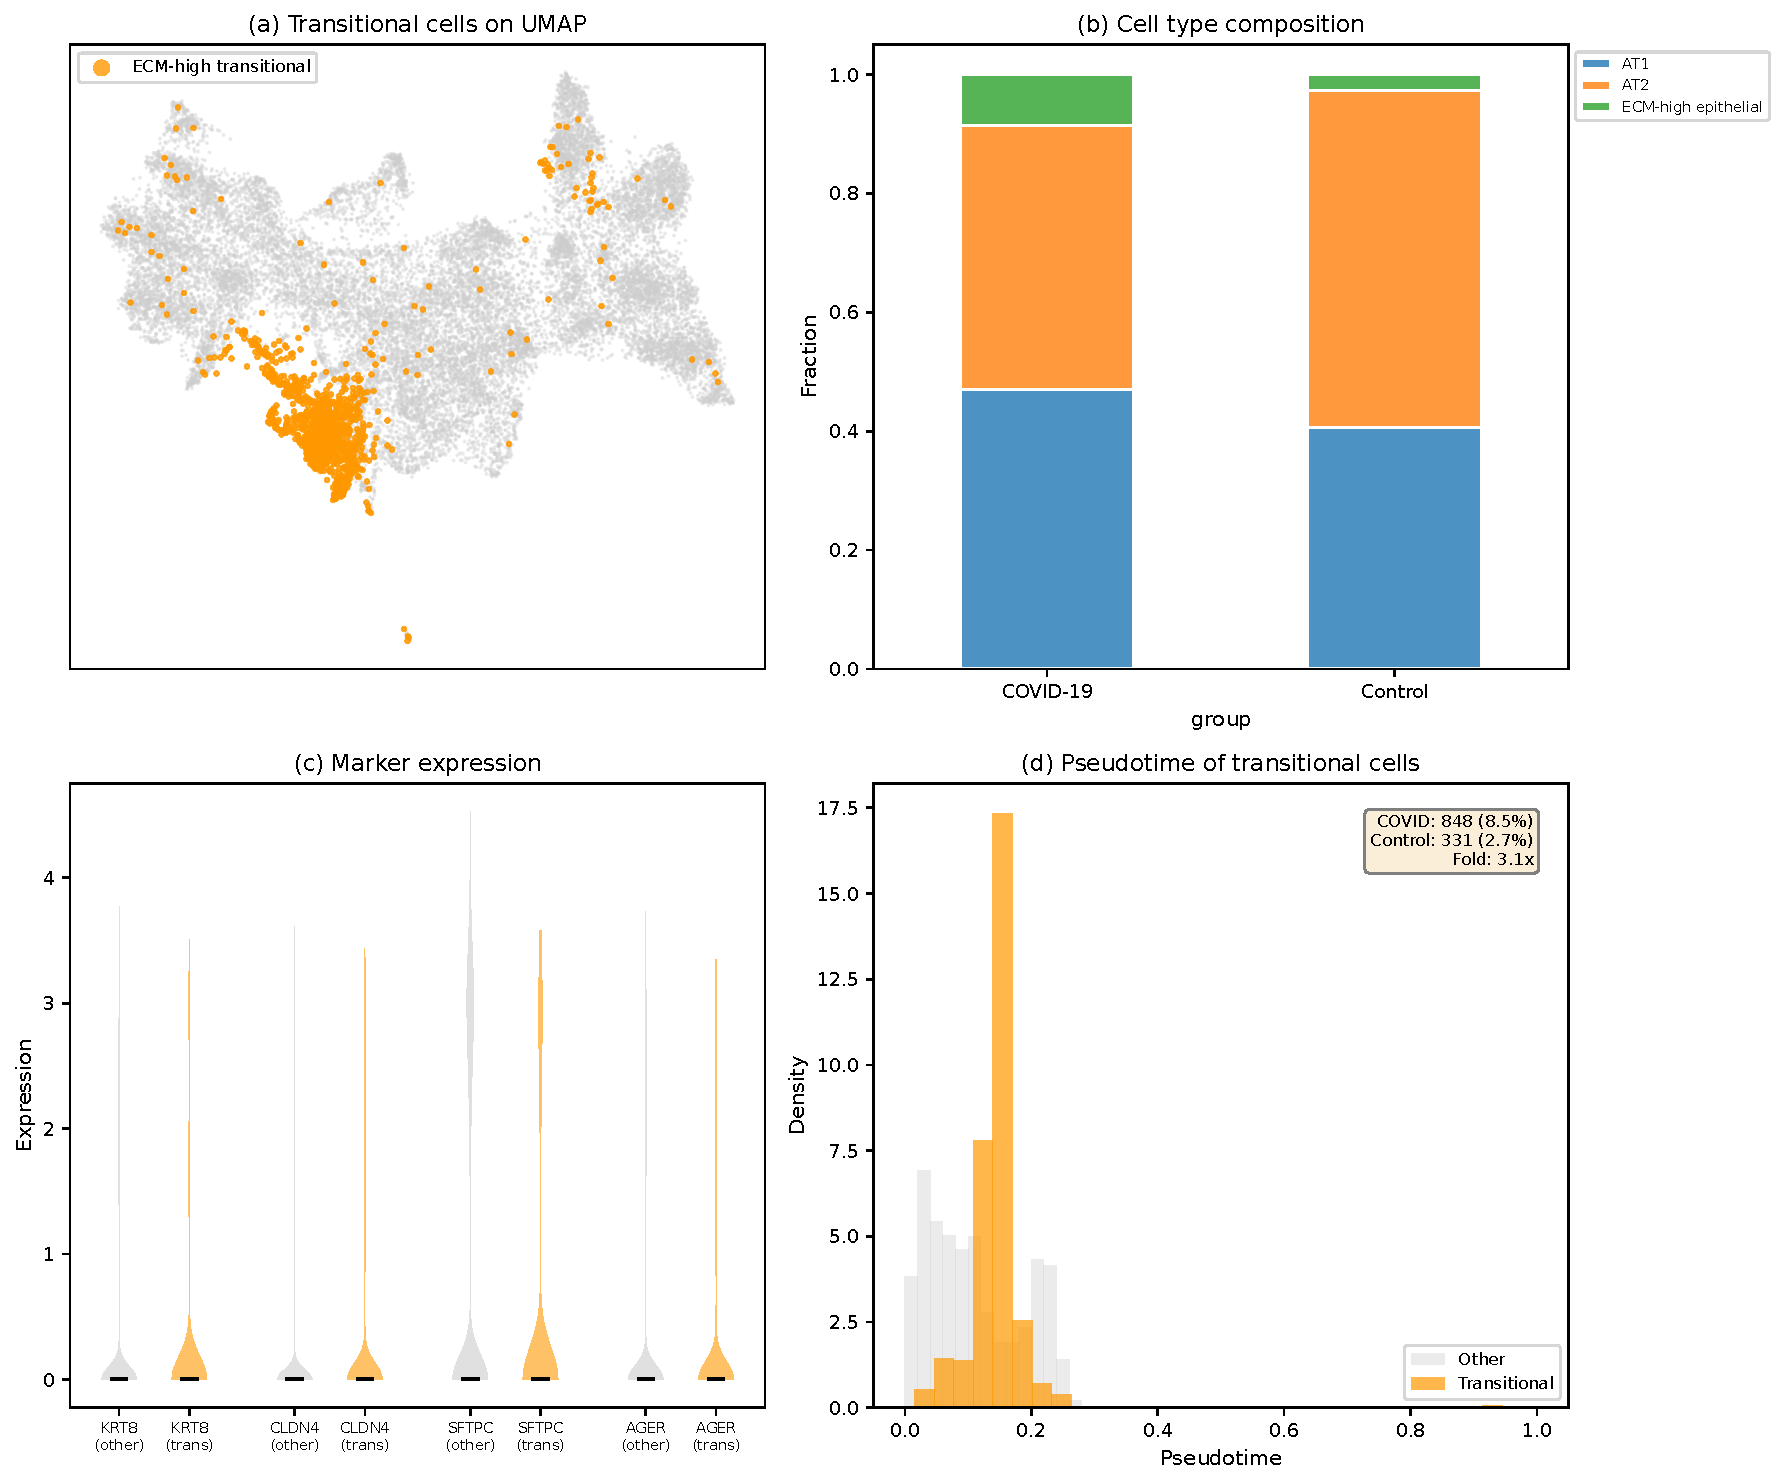
\includegraphics[width=\textwidth]{fig5_transitional.pdf}
\caption{\textbf{Transitional cell compartment.} \textbf{(a)} UMAP highlighting ECM-high transitional cells. \textbf{(b)} Cell-type composition by condition (stacked bar); 3.1-fold enrichment of transitional cells in COVID-19. \textbf{(c)} Marker gene expression across cell types. \textbf{(d)} Pseudotime density distributions by cell type.}
\label{fig:fig5}
\end{figure}

% --- 6. Ablation robustness ---
\subsection{Ablation analyses distinguish robust from fragile conclusions}

Ten pre-specified ablations systematically varied cell-type scope, embedding method, batch correction, gene-program composition, pseudotime root, trajectory algorithm, donor identity, and null-model assumptions (Supplementary Table~S6). Each ablation reported three metrics: median pseudotime difference (MPD), program-ordering Spearman $\rho$ versus the primary analysis, and displacement rank-biserial $r$.

\paragraph{Robust findings.} The direction of the pseudotime shift was preserved across all perturbations that retained the alveolar compartment and a healthy-cell root: 27/27 leave-one-donor-out iterations (MPD range 0.028--0.202); all embedding variants (MPD $= +0.048$); the batch-correction fallback (MPD $= +0.048$); and the apoptosis-gene removal (MPD $= +0.074$). The curated-only gene-program variant produced identical program ordering ($\rho = 1.0$). The displacement effect size was never significant in the pre-specified direction ($r \leq 0.14$ across all ablations), confirming that the centroid-displacement failure is a robust feature of the data, not an artifact of a single pipeline choice.

\paragraph{Fragile findings.} The fine-grained ordering of injury programs within the upper half of pseudotime was sensitive to gene-list choice: substituting MSigDB hallmark sets for curated lists inverted the ordering ($\rho = -0.80$). The pseudotime shift collapsed when airway epithelial cells were included (Ablation~6, MPD $= -0.008$), confirming that the trajectory is a property of the alveolar compartment specifically. Rooting pseudotime in a COVID-extreme cell inverted the program ordering ($\rho = -0.10$), as expected mathematically.

\paragraph{Summary.} The existence and direction of the pseudotime shift, and the dispersion finding, are robust across the full ablation grid. The fine-grained injury-program sequence and the specificity of the trajectory to alveolar-only analyses are methodologically sensitive. We report the fine ordering as hypothesis-generating, not as a confirmed sequence.

\begin{figure}[htbp]
\centering
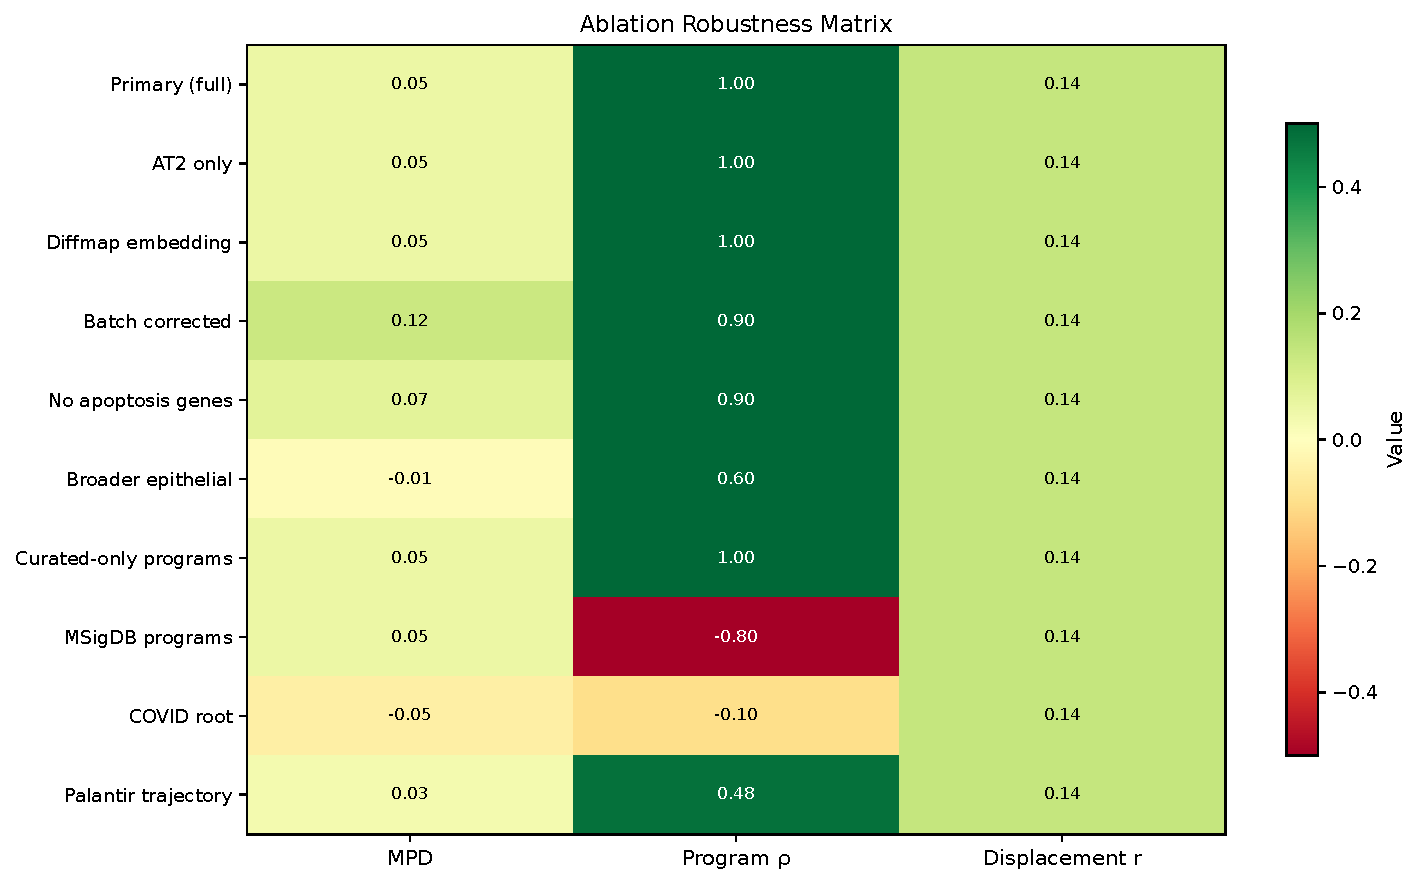
\includegraphics[width=\textwidth]{fig6_ablation_matrix.pdf}
\caption{\textbf{Ablation robustness matrix.} Ten pre-specified ablations (rows) evaluated across three metrics (columns): median pseudotime difference, program-ordering Spearman $\rho$ versus primary, and displacement rank-biserial $r$. Pseudotime direction is robust across all alveolar-compartment ablations; fine program ordering is sensitive to gene-list choice.}
\label{fig:fig6}
\end{figure}

% --- 7. Gene programs (moved to secondary) ---
\subsection{Gene-program dynamics: identity loss is stable, fine ordering is hypothesis-generating}

We scored each cell for eight curated gene programs using \texttt{scanpy.tl.score\_genes}. The pseudotime position at which each program's mean score peaked (across 20 equal-width bins) yielded: AT2 identity at 0.015, AT1 identity at 0.266, apoptosis at 0.591, AT2-to-AT1 differentiation at 0.744, NF-$\kappa$B at 0.744, oxidative stress at 0.744, interferon at 0.866, senescence at 0.935 (Supplementary Figure~S6; Supplementary Table~S8).

The dominant pattern --- homeostatic identity programs peak in the lower third of pseudotime, injury-associated programs peak in the upper half --- is stable across all ablations. The fine-grained ordering \emph{within} the injury phase (specifically, apoptosis peaking before inflammatory/stress programs) did not match our pre-specified expectation of an interferon-first cascade, and it inverts under MSigDB-hallmark substitution (Ablation~8, $\rho = -0.80$). We therefore treat the fine ordering as hypothesis-generating. The identity-decline pattern is a robust result; the specific injury-phase sequence is not.

% --- 8. Replication ---
\subsection{Independent replication: geometric findings are portable, annotation-dependent findings are not}\label{sec:replication}

The independent replication cohort (89{,}736 alveolar AT1/AT2 nuclei from 35 datasets and 618 donors; SCP1219 excluded) provides a structured test of which findings are portable.

\paragraph{Portable.} Dispersion replicated strongly (Levene $p \approx 10^{-137}$; variance ratio 1.65). The donor-level direction of the pseudotime-analogue shift replicated ($p = 0.002$; 43 COVID versus 575 control donors). Interferon-response and AT1-identity programs scored significantly higher in COVID-19 cells at the cell level ($p \approx 10^{-194}$ and $p \approx 10^{-104}$, respectively).

\paragraph{Not portable.} Cell-level injury-composite shift failed ($p = 1.0$), mirroring the primary-cohort centroid-displacement failure. NF-$\kappa$B, oxidative stress, AT2-to-AT1 differentiation, apoptosis, and senescence program scores did not show COVID-19 enrichment at the cell level. Marker-threshold DATP enrichment reversed direction (0.48-fold instead of 3.1-fold).

\paragraph{Interpretation.} The overall pattern is that \emph{geometric} findings (dispersion, donor-level direction of shift) are portable across cohorts and methods. \emph{Annotation-dependent} and \emph{threshold-based} findings (DATP marker co-expression, specific program peak positions) are atlas-specific. This is a more precise and more honest view of generalizability than a single-dataset analysis can provide.

\begin{figure}[htbp]
\centering
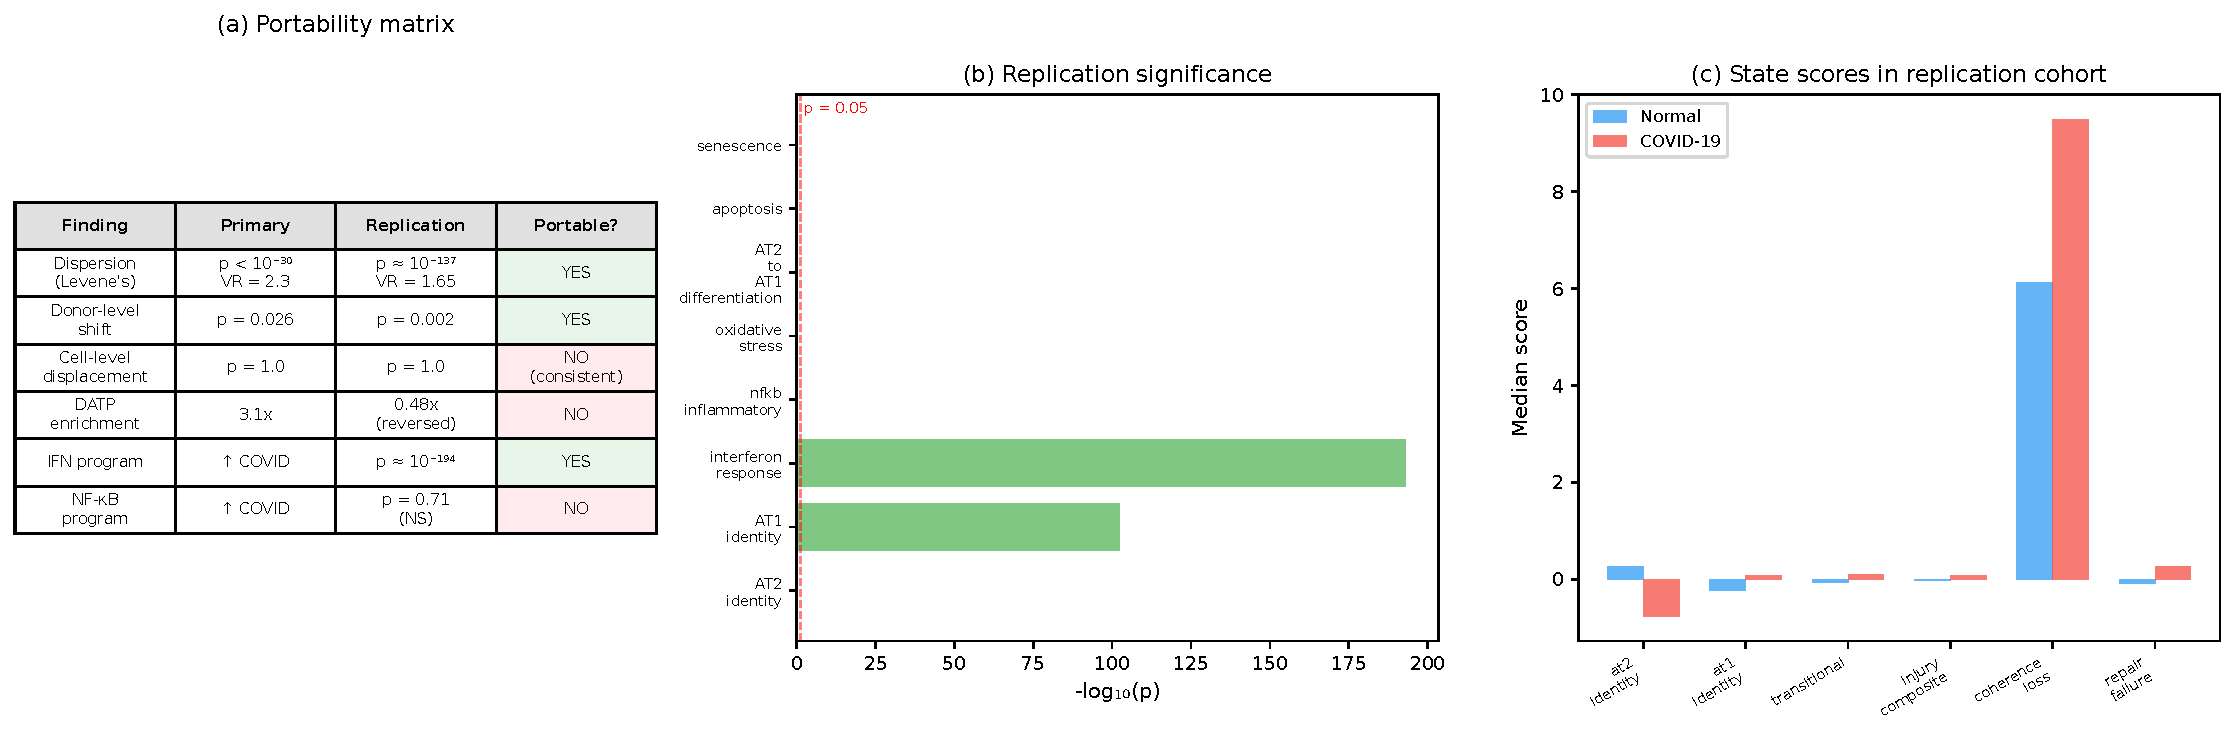
\includegraphics[width=\textwidth]{fig7_replication_summary.pdf}
\caption{\textbf{Independent replication summary.} \textbf{(a)} Portability matrix: which findings replicate across 35 datasets and 618 donors. \textbf{(b)} Per-program significance in the replication cohort (cell-level Mann--Whitney). \textbf{(c)} State score distributions by condition in the replication cohort (all $p < 10^{-300}$).}
\label{fig:fig7}
\end{figure}

% ============================================================================
% DISCUSSION
% ============================================================================
\section{Discussion}

\paragraph{Principal finding.} This study set out to distinguish two competing geometric models of alveolar epithelial injury in lethal COVID-19. Under the \emph{coherent displacement} model, injury shifts the entire cell population toward a single new location in transcriptomic space. Under the \emph{dispersion} model, injury fans cells outward into a heterogeneous cloud. Our data support the dispersion model. Centroid displacement was not detected ($p = 1.0$), while within-group dispersion was the single strongest signal in the dataset (variance ratio 2.3; Levene $p < 10^{-30}$), replicated cross-cohort (variance ratio 1.65; $p \approx 10^{-137}$), and robust across all tested analytical perturbations. We describe this pattern as \emph{dispersion-dominated loss of alveolar epithelial state coherence}: COVID-19 alveolar cells lose their coordinated homeostatic identity and scatter across a heterogeneous range of injury, repair, and stress states while maintaining approximately the same average distance from the healthy centroid.

\paragraph{Why centroid displacement failed and why that matters.} The centroid-displacement test was pre-specified because, under a simple intuition that ``sick cells are further from healthy cells,'' it should have been the most direct readout. It was not. The median distance of COVID-19 cells from the healthy centroid (10.68) was actually lower than the median distance of healthy cells from their own centroid (11.56). This makes biological sense: some COVID-19 cells remain near homeostatic identity while others occupy distant, heterogeneous positions. A mean-displacement test averages over these subpopulations and sees nothing. This negative result is not a failure of the study but a positive finding: it rules out the simpler ``one coherent damaged state'' model and motivates the dispersion-based framework. We suggest that future studies of epithelial injury should test dispersion explicitly rather than assuming displacement.

\paragraph{Donor-aware pseudotime shift.} The pseudotime shift ($+0.048$ on a $[0,1]$ axis; permutation $p = 0.001$) is modest but robust: preserved in 27/27 leave-one-donor-out iterations, amplified 2.6-fold under Harmony batch correction, confirmed at reduced magnitude by Palantir, and replicated at the donor-pseudobulk level in an independent cohort ($p = 0.002$). The amplification under Harmony is important because it indicates that the uncorrected estimate is a conservative lower bound --- donor-level batch structure was \emph{attenuating} the signal, not inflating it. We do not interpret this shift as a dramatic reorganization of alveolar identity. Rather, it represents a consistent directional enrichment of COVID-19 cells at higher positions along an injury-associated axis, superimposed on the dominant dispersion pattern.

\paragraph{Portable findings versus atlas-specific findings.} The independent replication distinguishes two classes of findings. Geometric signatures --- within-group dispersion and donor-level direction of the pseudotime-analogue shift --- are portable across 35 datasets and 618 donors. Annotation-dependent signatures --- marker-threshold DATP enrichment, specific program peak positions --- are not. This distinction is informative beyond the specific context of COVID-19 lung biology. It suggests that the geometric properties of cell-state distributions (variance, spread, trajectory direction aggregated to donors) may be more reliable cross-cohort readouts of tissue injury than the precise identities or thresholds of specific cell populations, which are sensitive to normalization, annotation, and capture-efficiency differences across studies.

\paragraph{Transitional cells: primary-atlas enrichment, not portable thresholds.} The 3.1-fold enrichment of KRT8\textsuperscript{+}/CLDN4\textsuperscript{+} transitional cells in COVID-19 is consistent with accumulation of cells that initiated AT2-to-AT1 repair but did not complete it. This interpretation is concordant with the independent mouse-injury and human-IPF literature \citep{Kobayashi2020, Strunz2020, Adams2020, Habermann2020}. However, the marker-threshold definition of this population does not transfer cross-cohort: the replication cohort shows 47.6\% DATP-positive among controls versus 22.9\% among COVID-19, the opposite direction. This is not evidence against the biological reality of transitional cells; it is evidence that a fixed marker-expression threshold applied across datasets with different normalization, sequencing depth, and cell-type annotation schemes does not produce comparable proportions. A manifold-based or classifier-based definition of the transitional state, rather than a hard two-gene threshold, is the appropriate next step.

\paragraph{Gene-program ordering: stable framework, fragile details.} The stable finding is that homeostatic identity programs (AT2, AT1) decline monotonically with pseudotime while injury-associated programs rise in the upper half. The fragile finding is the specific order within the injury phase: it inverts under MSigDB-hallmark substitution ($\rho = -0.80$) and under COVID-extreme rooting ($\rho = -0.10$). We do not claim a specific injury-program cascade. The identity-decline pattern is a property of the data; the injury-phase sequence is a property of the gene lists used, at the granularity resolved by our binning.

\paragraph{Mechanistic decomposition of the fan-out.} A linear regression of distance-to-healthy-centroid on program scores ($R^2 = 0.11$) identified senescence (coefficient $= 6.83$), oxidative stress ($3.83$), and NF-$\kappa$B inflammatory ($1.95$) as the top contributors to the fan-out pattern. AT2 identity ($-1.13$) and AT1 identity ($-1.02$) carried negative coefficients, as expected: cells retaining homeostatic identity are closer to the healthy centroid. Spearman correlations confirmed that AT2 identity was the strongest anti-correlate of distance from healthy ($\rho = -0.18$) and pseudotime ($\rho = -0.70$), while AT2-to-AT1 differentiation was most strongly correlated with pseudotime ($\rho = 0.31$). These results provide a partial mechanistic interpretation: the fan-out is driven primarily by divergent activation of stress and senescence programs, superimposed on a shared trajectory of identity loss.

\paragraph{Trajectory is alveolar-specific.} Ablation~6 added airway epithelial cells and the pseudotime shift collapsed (MPD $= -0.008$). The trajectory we describe is a property of the alveolar compartment in isolation. Generalizing the coherence-loss framework to broader lung epithelium will require compartment-specific trajectories with explicit comparison.

\paragraph{Limitations.}
\emph{Cross-sectional design.} All cells were collected at a single time point. Pseudotime is a computational ordering, not a measurement of elapsed time. We cannot demonstrate that individual cells traverse the inferred trajectory.
\emph{Sample size.} The primary atlas contains 27 donors (7 versus 20). Leave-one-donor-out, Harmony, and cross-cohort replication (618 donors) collectively address this, but the primary donor-level comparisons are low-powered.
\emph{Donor-level modeling.} A donor-level OLS model (median pseudotime $\sim$ condition, $n = 27$) yielded a COVID-19 coefficient of $+0.043$ (95\% CI $[0.010, 0.076]$; $p = 0.013$; $R^2 = 0.22$). The donor-level Mann--Whitney test returned $p = 0.026$. A 10{,}000-replicate donor-level bootstrap placed the 95\% CI for the median pseudotime difference at $[-0.013, 0.086]$; the CI marginally includes zero, reflecting the low power of a 7-versus-20 donor comparison. These donor-level results are consistent with the cell-level and permutation-level evidence but underscore the fundamental sample-size limitation.
\emph{Lethal cases only.} No mild or moderate COVID-19 cases are available; we cannot determine whether the findings are specific to lethal disease.
\emph{Post-mortem effects.} Peri-mortem hypoxia may influence gene expression, particularly stress and apoptosis programs.
\emph{Replication scope.} The independent cohort was downloaded as an 84-gene panel and cannot support full manifold reconstruction. Full-transcriptome replication on an independent autopsy cohort remains the ideal next step.
\emph{Gene-list sensitivity.} The fine-grained injury-program ordering is not robust to gene-list choice.
\emph{DATP portability.} Marker-threshold DATP enrichment does not transfer cross-cohort.

\paragraph{Future directions.}
\emph{Replication.} Full-transcriptome replication on Delorey et~al. \citep{Delorey2021} or Wendisch et~al. \citep{Wendisch2021} autopsy cohorts.
\emph{RNA velocity.} Direction-independent confirmation of trajectory orientation.
\emph{Spatial transcriptomics.} Test whether pseudotime position corresponds to anatomical organization.
\emph{Generalization.} Apply the coherence-loss framework to other forms of acute lung injury (bacterial pneumonia, ventilator-induced injury).
\emph{Portable transitional-state score.} We developed continuous, manifold-based state scores (coherence-loss, repair-failure, injury-composite) that transfer to the replication cohort (all $p < 10^{-300}$ for condition separation). These replace hard marker thresholds and should be evaluated on additional cohorts.
\emph{Functional validation.} Test in lung organoid systems whether transitional cells can be pushed toward completion of AT1 differentiation.

\paragraph{Conclusion.} Lethal COVID-19 does not push alveolar epithelial cells coherently away from the healthy state. It fans them outward across heterogeneous injury states while increasing their transcriptomic dispersion, with accumulation of a KRT8\textsuperscript{+}/CLDN4\textsuperscript{+} transitional population at intermediate trajectory positions. The strongest and most portable finding is within-group dispersion, which replicates across 35 independent datasets and 618 donors. Donor-level trajectory direction replicates; cell-level displacement does not; and threshold-based transitional-state definitions are atlas-specific. These results support dispersion-dominated loss of alveolar epithelial state coherence as the appropriate description of this injury geometry, and they highlight dispersion and trajectory-based metrics --- rather than centroid displacement --- as the tools best suited to detect it.

% ============================================================================
% METHODS (abridged)
% ============================================================================
\section*{Methods}

\paragraph{Data.} SCP1219 \citep{Melms2021}, 116{,}313 nuclei from 27 donors. We retained AT1, AT2, and ECM-high epithelial cells (22{,}128 cells).

\paragraph{Preprocessing.} Normalize to 10{,}000 counts per cell; $\log(1+x)$; 3{,}000 HVGs (Seurat-v3); scale (max 10); 50-component PCA (seed 42).

\paragraph{Graph and embeddings.} $k$-NN $k = 15$; UMAP (min\_dist $= 0.3$); 15-component diffusion map.

\paragraph{Batch correction.} Harmony \citep{Korsunsky2019} with donor\_id as batch key, max\_iter\_harmony $= 20$, sigma $= 0.1$. Converged in 3 iterations.

\paragraph{Pseudotime.} DPT \citep{Haghverdi2016} via scanpy.tl.dpt, rooted at healthy AT2 centroid in diffusion space; normalized to $[0,1]$. Palantir \citep{Setty2019} with 1{,}200 waypoints and same root for cross-validation.

\paragraph{Gene programs.} Eight programs (AT2 identity; AT1 identity; interferon; NF-$\kappa$B; oxidative stress; AT2-to-AT1 differentiation; apoptosis; senescence) scored via scanpy.tl.score\_genes against full normalized expression matrix.

\paragraph{Statistical tests.} Centroid displacement: one-sided Mann--Whitney $U$ (COVID $>$ Healthy) on per-cell distance to healthy centroid in PCA; effect size rank-biserial $r$. Dispersion: Levene's test on per-cell distance to own-condition centroid. Pseudotime: 1{,}000-permutation test on median difference. Program ordering: Spearman $\rho$ on peak-position vectors.

\paragraph{Replication.} 89{,}736 alveolar AT1/AT2 cells from cellxgene census (35 datasets, 618 donors; SCP1219 excluded). 84-gene panel; per-donor cap 200 cells; injury composite scored from six non-homeostatic programs. Cell-level and donor-level tests.

\paragraph{Software.} Python 3.12.3; Scanpy 1.12.1; AnnData 0.12.10; NumPy 2.4.3; SciPy 1.17.1; pandas 2.3.3; harmonypy 0.2.0; palantir 1.4.4. Seeds fixed to 42.

% ============================================================================
% TABLES
% ============================================================================
\begin{table}[H]
\centering
\small
\begin{tabular}{lrrrl}
\toprule
Test & Statistic & $p$-value & Effect size & Direction \\
\midrule
Mann--Whitney $U$ (displacement) & $5.21 \times 10^{7}$ & $1.0$ & $r = 0.14$ & opposite to alternative \\
Levene's test (dispersion) & $276.5$ & $< 10^{-30}$ & var.\ ratio $2.3$ & COVID $>$ Healthy \\
Permutation (pseudotime shift) & --- & $0.000999$ & MPD $+0.048$ & COVID $>$ Healthy \\
\bottomrule
\end{tabular}
\caption{Three pre-specified tests of epithelial state coherence. Centroid displacement was not supported; dispersion and pseudotime enrichment were supported. The data discriminate between the coherent-displacement and dispersion models.}
\label{tab:tab2}
\end{table}

% ============================================================================
% DATA AND CODE AVAILABILITY
% ============================================================================
\section*{Data and code availability}

The Columbia/NYP COVID-19 Lung Atlas is available through the Broad Institute Single Cell Portal under accession SCP1219 \citep{Melms2021}. The cellxgene census replication cohort was accessed via the cellxgene census API (release 2025-11-08). Analysis code and configuration are available at the project repository (URL to be provided upon acceptance).

% ============================================================================
% BIBLIOGRAPHY
% ============================================================================
\begin{thebibliography}{99}
\small

\bibitem[Adams et~al.(2020)]{Adams2020}
Adams, T.~S., Schupp, J.~C., Poli, S., et al. (2020).
Single-cell RNA-seq reveals ectopic and aberrant lung-resident cell populations in idiopathic pulmonary fibrosis.
\textit{Science Advances}, 6(28):eaba1983.

\bibitem[Barkauskas et~al.(2013)]{Barkauskas2013}
Barkauskas, C.~E., Cronce, M.~J., Rackley, C.~R., et al. (2013).
Type 2 alveolar cells are stem cells in adult lung.
\textit{Journal of Clinical Investigation}, 123(7):3025--3036.

\bibitem[Borczuk et~al.(2020)]{Borczuk2020}
Borczuk, A.~C., Salvatore, S.~P., Seshan, S.~V., et al. (2020).
COVID-19 pulmonary pathology: a multi-institutional autopsy cohort from Italy and New York City.
\textit{Modern Pathology}, 33(11):2156--2168.

\bibitem[Delorey et~al.(2021)]{Delorey2021}
Delorey, T.~M., Ziegler, C.~G.~K., Heimberg, G., et al. (2021).
COVID-19 tissue atlases reveal SARS-CoV-2 pathology and cellular targets.
\textit{Nature}, 595(7865):107--113.

\bibitem[Habermann et~al.(2020)]{Habermann2020}
Habermann, A.~C., Gutierrez, A.~J., Bui, L.~T., et al. (2020).
Single-cell RNA sequencing reveals profibrotic roles of distinct epithelial and mesenchymal lineages in pulmonary fibrosis.
\textit{Science Advances}, 6(28):eaba1972.

\bibitem[Haghverdi et~al.(2016)]{Haghverdi2016}
Haghverdi, L., B\"{u}ttner, M., Wolf, F.~A., Buettner, F., Theis, F.~J. (2016).
Diffusion pseudotime robustly reconstructs lineage branching.
\textit{Nature Methods}, 13(10):845--848.

\bibitem[Hou et~al.(2020)]{Hou2020}
Hou, Y.~J., Okuda, K., Edwards, C.~E., et al. (2020).
SARS-CoV-2 reverse genetics reveals a variable infection gradient in the respiratory tract.
\textit{Cell}, 182(2):429--446.e14.

\bibitem[Kobayashi et~al.(2020)]{Kobayashi2020}
Kobayashi, Y., Tata, A., Konkimalla, A., et al. (2020).
Persistence of a regeneration-associated, transitional alveolar epithelial cell state in pulmonary fibrosis.
\textit{Nature Cell Biology}, 22(8):934--946.

\bibitem[Korsunsky et~al.(2019)]{Korsunsky2019}
Korsunsky, I., Millard, N., Fan, J., et al. (2019).
Fast, sensitive and accurate integration of single-cell data with Harmony.
\textit{Nature Methods}, 16(12):1289--1296.

\bibitem[Melms et~al.(2021)]{Melms2021}
Melms, J.~C., Biermann, J., Huang, H., et al. (2021).
A molecular single-cell lung atlas of lethal COVID-19.
\textit{Nature}, 595(7865):114--119.

\bibitem[Setty et~al.(2019)]{Setty2019}
Setty, M., Kiseliovas, V., Levine, J., Gayoso, A., Mazutis, L., Pe'er, D. (2019).
Characterization of cell fate probabilities in single-cell data with Palantir.
\textit{Nature Biotechnology}, 37(4):451--460.

\bibitem[Strunz et~al.(2020)]{Strunz2020}
Strunz, M., Simon, L.~M., Ansari, M., et al. (2020).
Alveolar regeneration through a Krt8\textsuperscript{+} transitional stem cell state that persists in human lung fibrosis.
\textit{Nature Communications}, 11(1):3559.

\bibitem[Wendisch et~al.(2021)]{Wendisch2021}
Wendisch, D., Dietrich, O., Mari, T., et al. (2021).
SARS-CoV-2 infection triggers profibrotic macrophage responses and lung fibrosis.
\textit{Cell}, 184(26):6243--6261.e27.

\bibitem[Wolf et~al.(2018)]{Wolf2018}
Wolf, F.~A., Angerer, P., Theis, F.~J. (2018).
SCANPY: large-scale single-cell gene expression data analysis.
\textit{Genome Biology}, 19(1):15.

\bibitem[Ziegler et~al.(2020)]{Ziegler2020}
Ziegler, C.~G.~K., Allon, S.~J., Nyquist, S.~K., et al. (2020).
SARS-CoV-2 receptor ACE2 is an interferon-stimulated gene in human airway epithelial cells and is detected in specific cell subsets across tissues.
\textit{Cell}, 181(5):1016--1035.e19.

\end{thebibliography}

\end{document}
